\section{Preissmann scheme}\label{subse:preissmann_scheme}
In this section, the Saint Venant equations are solved using a numerical method.

%Argument for at bruge numeriske metode til at løse saint venant eq.

The numerical method used for solving the Saint Venant equations, described in section \ref{se:hydraulics_of_sewer_line}, is the Preissmann scheme which is based on the box scheme. Other methods exist such as Lax scheme, Abbot-Ionescu scheme, leap-frog scheme, Vasiliev scheme, however, the Preissmann scheme is commonly known as the most robust. Basically, by using the Preissmann scheme the Saint Venant equations can be discretized, and thereby utilized to simulate the flow and height throughout an open channel.

From section \ref{se:hydraulics_of_sewer_line} the Saint Venant equations for conservation of mass and momentum are derived, they are also shown below.

\begin{equation}\label{eq:saintbernard_mass_preiss}
\frac{\partial A(x,t)}{\partial t} + \frac{\partial Q(x,t)}{\partial x}=0
\end{equation}

\begin{equation}\label{eq:saintbernard_momentum_preiss}
\frac{1}{gA} \frac{\partial Q}{\partial t} +\frac{1}{gA}\frac{\partial}{\partial x} \left( \frac{Q^2}{A} \right) + \frac{\partial h}{\partial x} + S_f - S_b = 0
\end{equation}

%Skriv noget om boundary og initial conditions

In figure \ref{fig:preissmann_grid_scheme} a single mesh for the Preissmann scheme is illustrated.

\begin{figure}[H]
\centering
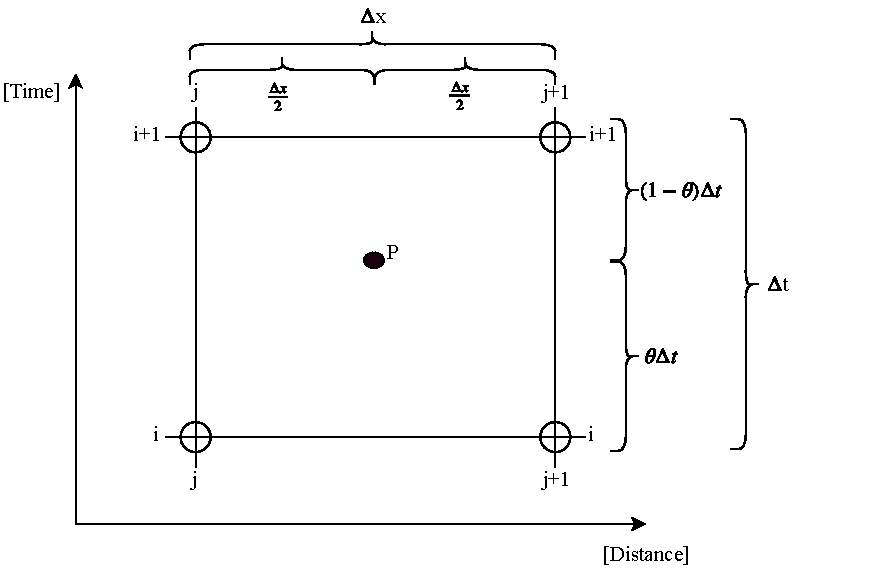
\includegraphics[width=.6\textwidth]{report/simulation/pictures/preissmann_scheme}
\caption{Preissmann non-staggered grid scheme.}
\label{fig:preissmann_grid_scheme}
\end{figure}

Where $\theta$ is a weighting parameter ranging between zero and one, j is an index of cross section and i is an index of time. The mesh contains four nodes, (j,i), (j+1,i), (j,i+1) and (j+1,i+1), however in the implementation the dimension of the grid is $\Delta t \times \Delta x$ for $0 \leq x \leq L$ and $0\leq t$. Where L defines the length of the open channel section. The derivatives in equations \ref{eq:saintbernard_mass_preiss} and \ref{eq:saintbernard_momentum_preiss} are calculated as an approximation at the point P, which is in the middle of the interval of $\Delta x$.% and is also the reason why the Preissmann scheme is corresponding to a box scheme.
The difference between the box scheme and the Preissmann scheme is that the point P is always found at the middle of $\Delta x$ and the point can only move along the time axis within this mesh by adjusting the weighting parameter $\theta$. This weighting parameter will be elaborated on later. An arbitrary function $f_p(x,t)$ calculated at point P is approximated by \cite{numerical_modeling}.

\begin{equation}\label{eq:approximated_function}
	f_P \approx \frac{1}{2} (\theta \cdot f_j^{i+1}+(1-\theta)f_j^i)+\frac{1}{2}(\theta\cdot f_{j+1}^{i+1}+(1-\theta)f_{j+1}^i)
\end{equation}
The numerical approximation for the derivatives in equations \ref{eq:saintbernard_mass_preiss} and \ref{eq:saintbernard_momentum_preiss} for time and length are shown below \cite{numerical_modeling}.

\begin{equation}\label{eq:preissmann_time_derivatie}
	\frac{\partial f}{\partial t}\bigg \rvert_P \approx \frac{1}{2}\left(\frac{f_j^{i+1}-f_j^i}{\Delta t}+\frac{f_{j+1}^{i+1}-f_{j+1}^i}{\Delta t}\right)
\end{equation}

\begin{equation}\label{eq:preissmann_space_derivatie}
	\frac{\partial f}{\partial x}\bigg \rvert_P \approx (1-\theta)\frac{f_{j+1}^i-f_{j}^i}{\Delta x}+\theta \frac{f_{j+1}^{i+1}-f_{j}^{i+1}}{\Delta x}
\end{equation}

These approximations from equations \ref{eq:preissmann_time_derivatie} and \ref{eq:preissmann_space_derivatie} can therefore be inserted for the derivatives in the Saint Venant equations \ref{eq:saintbernard_mass_preiss} and \ref{eq:saintbernard_momentum_preiss} and thereby achieve the following,

\begin{equation}\label{eq:continuity_eq_preissmann}
	\theta \frac{Q_{j+1}^{i+1}-Q_j^{i+1}}{\Delta x}+(1-\theta)\frac{Q_{j+1}^i - Q_j^i}{\Delta x}+
	\frac{1}{2}\frac{A_{j+1}^{i+1}-A_{j+1}^i}{\Delta t} + \frac{1}{2} \frac{A_{j}^{i+1} - A_j^i}{\Delta t} = 0
\end{equation}

% \begin{multline}
% 	\frac{1}{2} \left(\frac{Q_{j+1}^{i+1}-Q_{j+1}^i}{\Delta t}+\frac{Q_{j}^{i+1} - Q_j^i}{\Delta t}\right) + \frac{\theta}{\Delta x} \left(\left(\frac{Q^2}{A}\right)_{j+1}^{i+1}-\left(\frac{Q^2}{A}\right)_{j}^{i+1}\right) + \\ \frac{1-\theta}{\Delta x}\left(\left(\frac{Q^2}{A}\right)_{j+1}^{i}-\left(\frac{Q^2}{A}\right)_{j}^{i}\right)+gA_p\theta \left(\frac{h_{j+1}^{i+1}-h_j^{i+1}}{\Delta x}\right)+ \\ gA_p(1-\theta)\left(\frac{h_{j+1}^{i} - h_j^i}{\Delta x}\right)+\left(\frac{g\cdot n_M^2}{R^\frac{4}{3}}\frac{|Q|Q}{A}\right)_P = 0
% \end{multline}
\begin{multline}
	\frac{1}{gA_p}\left(\frac{1}{2} \left(\frac{Q_{j+1}^{i+1}-Q_{j+1}^i}{\Delta t}+\frac{Q_{j}^{i+1} - Q_j^i}{\Delta t}\right)\right) + \frac{1}{gA_p}\left(\frac{\theta}{\Delta x} \left(\left(\frac{Q^2}{A}\right)_{j+1}^{i+1}-\left(\frac{Q^2}{A}\right)_{j}^{i+1}\right)\right) + \\ \frac{1-\theta}{\Delta x}\left(\left(\frac{Q^2}{A}\right)_{j+1}^{i}-\left(\frac{Q^2}{A}\right)_{j}^{i}\right)+\theta \left(\frac{h_{j+1}^{i+1}-h_j^{i+1}}{\Delta x}\right)+ \\ (1-\theta)\left(\frac{h_{j+1}^{i} - h_j^i}{\Delta x}\right)+S_f-S_b= 0
\end{multline}

By discretizing the Saint Venant equations they can be used in a simulation to calculate parameters for the open channel model. The mesh shown in figure \ref{fig:preissmann_grid_scheme} is used to calculate the node (j+1,i+1) by knowing the previous values in time and length (j,i), (j+1,i) and (j,i+1). Therefore some initial condition must be known to calculate the parameters for the open channel in the first iteration. The flow, at t=0, must be known throughout the pipe. Furthermore, the flow that will enter the channel for $t\leq 0$ must be known, as shown in figure \ref{fig:preissmann_grid_scheme_exampel}.

\begin{figure}[H]
\centering
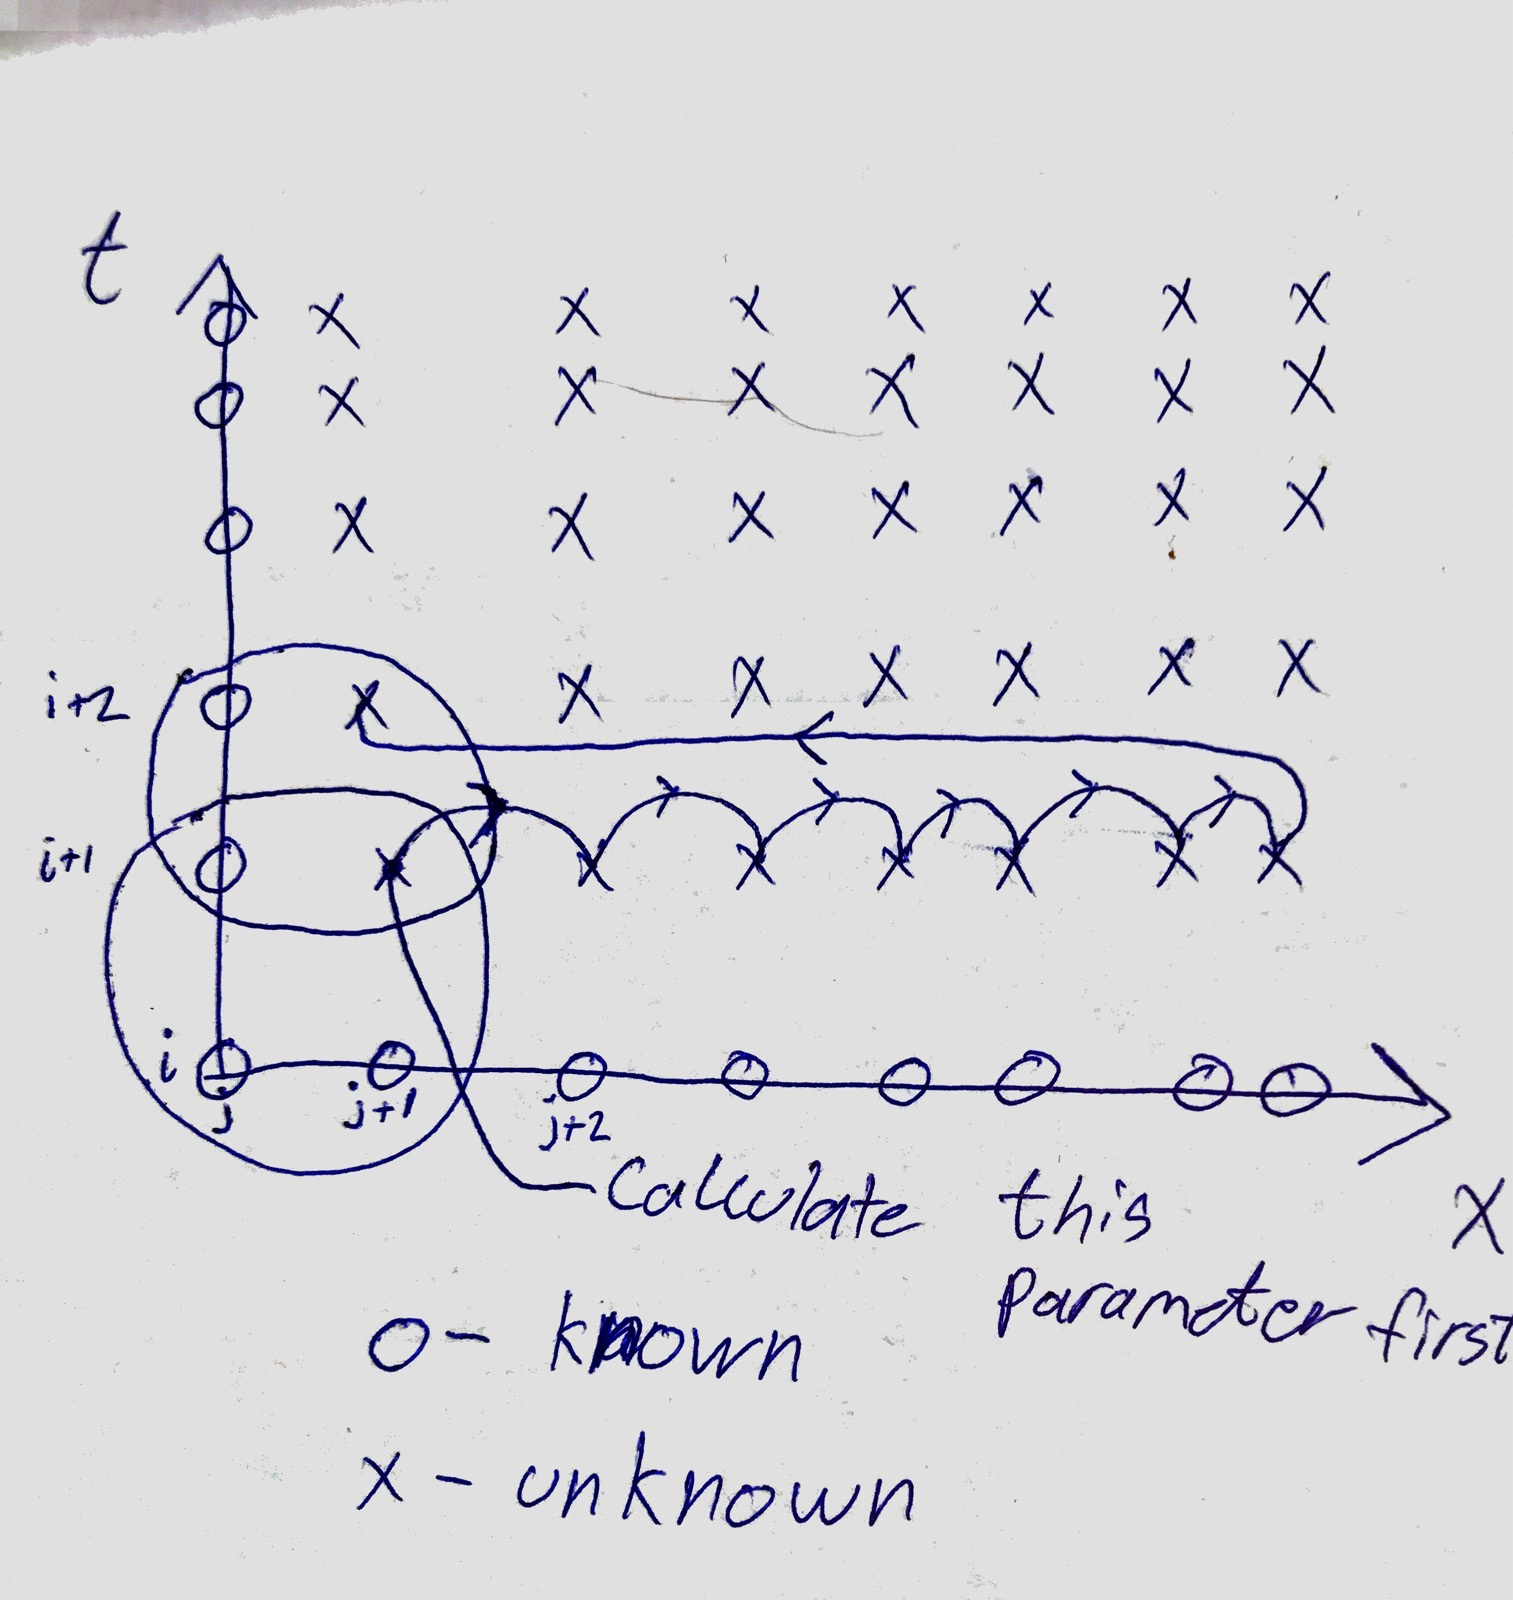
\includegraphics[width=.6\textwidth]{report/simulation/pictures/preissmann_scheme_exempel}
\caption{Preissmann non-staggered grid scheme example of calculation pattern.}
\label{fig:preissmann_grid_scheme_exampel}
\end{figure}
%% Dette skal omformuleres
By knowing the flow and parameters for the pipe, the height can be calculated in the initialization nodes, which will be elaborated on later. With equation \ref{eq:continuity_eq_preissmann}, the flow (j+1,i+1) can be calculated by knowing the flow and height in the previous nodes (j,i), (j+1,i) and (j,i+1) as illustrated with the box in the left bottom corner in figure \ref{fig:preissmann_grid_scheme_exampel}.

For the Preissmann scheme to be numerical stable the $\theta$ parameter is $\theta \leq 0,5$. Does closer $\theta$ is to 0,5 the more accurate it is, however it is also more likely to be unstable, therefore from \cite{theta_decision} it is suggested to place $\theta$ in the range of $0,55 \leq \theta \leq 0.65$ for practical analysis.

In the following section, the calculating of the flow and height in each node will be explained.

\subsubsection*{Iteration scheme}
In this section, it will be elaborated how the calculation of the flow and height in each iteration is done \cite{ikke_stationear}.

The discretized continuity equation \ref{eq:continuity_eq_preissmann} from section \ref{subse:preissmann_scheme}, stated below, is solved for the desired flow in equation \ref{eq:continuity_solve_flow},
\begin{equation}
	\theta \frac{Q_{j+1}^{i+1}-Q_j^{i+1}}{\Delta x}+(1-\theta)\frac{Q_{j+1}^i - Q_j^i}{\Delta x}+
	\frac{1}{2}\frac{A_{j+1}^{i+1}-A_{j+1}^i}{\Delta t} + \frac{1}{2} \frac{A_{j}^{i+1} - A_j^i}{\Delta t} = 0
\end{equation}

\begin{equation}\label{eq:continuity_solve_flow}
	Q_{j+1}^{i+1} = - \frac{1}{2\theta}\cdot\left(A_{j+1}^{i+1}-H\right)\cdot\frac{\Delta x}{\Delta t}
\end{equation}
Where H is a parameter for the previous flows and areas in time and section which are known as these are either been set to a specific input at time 0 to t and throughout the pipe, for t=0 as shown in figure \ref{fig:preissmann_grid_scheme_exampel} or has been calculated as the scheme have been iterated.
\begin{equation}
	H = \left(2\cdot(1-\theta)\cdot Q_j^i-2\cdot(1-\theta)\cdot Q_{j+1}^i+2\theta Q_j^{i+1}\right)\cdot\frac{\Delta t}{\Delta x}- A_{j}^{i+1}+A_j^i+A_{j+1}^i
\end{equation}

Instead of using the the second saint venant equation as explained in ??? \fxnote{ref tilbage til hvor vi vaelger den fra} an equation for calculating the flow in a circular pipe will be used:

\begin{equation}\label{eq:calc_for_flowv2}
 	Q = \left(0.46-0.5 \cdot cos\left(\pi \frac{h}{d}\right)+0.04\cdot cos\left(2\pi\frac{h}{d}\right)\right)\cdot Q_f
\end{equation}

This equation describes the flow in a circular pipe by knowing the diameter, d height, h and the flow for a filled pipe $Q_f$. Where $Q_f$ is calculated as:

\begin{equation}\label{eq:qf_for_flow}
	Q_f =-72\cdot \left(\frac{d}{4}\right)^{0.635}\pi\cdot\left(\frac{d}{2}\right)^2\cdot I_e^{0,5}% -3.02 \cdot ln\left(\frac{0.74\cdot 10^{-6}}{d\sqrt{d\cdot I_e}}+\frac{k}{3.71\cdot d}\right)d^2\sqrt{d\cdot I_e}
\end{equation}
$Q_f$ is calculated from Mannings eqaution and can be seen in appendix \ref{app:formulas}. Where $I_e$ is a friction term. \fxnote{skal der skrives her, at det er antaget at friction er lig med haeldning?}  \fxnote{lav hjaelpe formeller}

In equation \ref{eq:continuity_solve_flow} the flow $Q_{j+1}^{i+1}$ is a function of the unknown area $A_{j+1}^{i+1}$, and by subtracting the flow on each side the following is achieved,

\begin{equation}\label{eq:continuity_zero_eq}
		0=-Q_{j+1}^{i+1}  - \frac{1}{2\theta}\cdot\left(A_{j+1}^{i+1}-H\right)\cdot \frac{\Delta x}{\Delta t}
\end{equation}
By calling the right hand side of equation \ref{eq:continuity_zero_eq} for V the following is obtained,

\begin{equation}\label{eq:continuity_V}
		V=-Q_{j+1}^{i+1}  - \frac{1}{2\theta}\cdot\left(A_{j+1}^{i+1}-H\right)\cdot \frac{\Delta x}{\Delta t}
\end{equation}

Equation \ref{eq:continuity_V} can now be solved by finding the zero for the function V using newton method. However there are still two unknowns in equation \ref{eq:continuity_V}, $Q_{j+1}^{i+1}$ and $A_{j+1}^{i+1}$. $Q_{j+1}^{i+1}$ can be replaced with equation \ref{eq:calc_for_flowv2} for calculating the flow.

% \begin{equation}\label{eq:calc_for_flow}
%  	Q = \left(0.46-0.5 \cdot cos\left(\pi \frac{h}{d}\right)+0.04\cdot cos\left(2\pi\frac{h}{d}\right)\right)\cdot Q_f
% \end{equation}
% Which describes the flow in an open channel by knowing the height, diameter of the pipe and the flow for a fully filled pipe, $Q_f$.
%Where k is a roughness factor found in?? \fxnote{kilde til hvor vi finder den} and $I_e$ is a friction term.  
Equation \ref{eq:calc_for_flowv2} is inserted into equation \ref{eq:continuity_V} and thereby the following is obtained,

\begin{equation}\label{eq:V_with_flow}
	V = -Q_f\cdot\left(0,46-0,5\cdot cos\left(\pi \frac{h_{j+1}^{i+1}}{d}\right)+0,04\cdot cos\left(2\pi\frac{h_{j+1}^{i+1}}{d}\right)\right)\frac{\Delta t}{\Delta x}-\frac{1}{2\theta}\left(A_{j+1}^{i+1}-H\right)
\end{equation}

Furthermore $Q_f$ from equation \ref{eq:qf_for_flow} is inserted into equation \ref{eq:V_with_flow},

\begin{multline}\label{eq:new_continuity_equation}
	V = -72\left(\frac{d}{4}\right)^{0.635}\pi\cdot\left(\frac{d}{2}\right)^2I_e^{0,5}\cdot \left(0,46-0,5\cdot cos\left(\pi \frac{h_{j+1}^{i+1}}{d}\right)+ 0,04\cdot cos\left(2\pi\frac{h_{j+1}^{i+1}}{d}\right)\right)\\ \frac{\Delta t}{\Delta x}-\frac{1}{2\theta}\left(A_{j+1}^{i+1}-H\right)
\end{multline}

V is now a function of the height $h_{j+1}^{i+1}$ as the height is the only unknown in finding the area $A_{j+1}^{i+1}$ and the flow for the channel. The area for a circular channel is calculated with the following,

\begin{equation}\label{eq:calc_area_open_channel}
	A = \frac {d^2}{4} \cdot acos \left(\frac{\frac{d}{2}-h}{\frac{d}{2}}\right)-\sqrt{h\cdot (d-h)}\cdot  \left(\frac{d}{2}-h\right)
\end{equation}

As mention the continuity equation \ref{eq:new_continuity_equation} can be solved by finding the zero for the function V. Newtons method is used to find approximations to the roots/zeros of a real-valued function. By using the Newton method the roots of equation \ref{eq:new_continuity_equation} can be found, which will correspond to the height of the channel. The approximation is,

\begin{equation}
	 (h_{j+1}^{i+1})_{k+1} =(h_{j+1}^{i+1})_{k} - \frac{V_k}{V'_k}
\end{equation}

Where k is the number of iterations, V$'$ is the differentiated of V with respect to height, $(h_{j+1}^{i+1})_{k}$ is an initial guess of the root and $(h_{j+1}^{i+1})_{k+1}$ is a better approximation of the height. This calculation is iterated until a satisfied approximation is achieved which fulfills the requirement,

\begin{equation}
	\left(h_{j+1}^{i+1}\right)_{k}-(h_{j+1}^{i+1})_{k-1} < (\epsilon \cdot h_{j+1}^{i+1})_{k}
\end{equation}

Where $\epsilon$ is a small tolerance number, e.g. 5-centimeter variation in water height. Thereby the water height can be found and the area of the water can be calculated with equation \ref{eq:calc_area_open_channel} \fxnote{afsnit om de forskellige ligninger til beregning af Areal, Ie,Ib,Qf,Q} and thereafter equation \ref{eq:continuity_solve_flow} can be used to calculate the flow of the node.

This calculation is performed for each node in the Preissmann scheme, therefore it is an iterative method of solving the flow for an open channel and in figure ??? an illustration of how these equations are iterated is shown.


In the following figures the flow \ref{fig:simulation_output_flow_height_a} and the water height \ref{fig:simulation_output_flow_height_b} for the output of the channel is plotted


\begin{figure}[H]
\centering
\begin{subfigure}{.5\textwidth}
  \centering
  % This file was created by matlab2tikz.
%
%The latest updates can be retrieved from
%  http://www.mathworks.com/matlabcentral/fileexchange/22022-matlab2tikz-matlab2tikz
%where you can also make suggestions and rate matlab2tikz.
%
\definecolor{mycolor1}{rgb}{0.00000,0.44700,0.74100}%
%
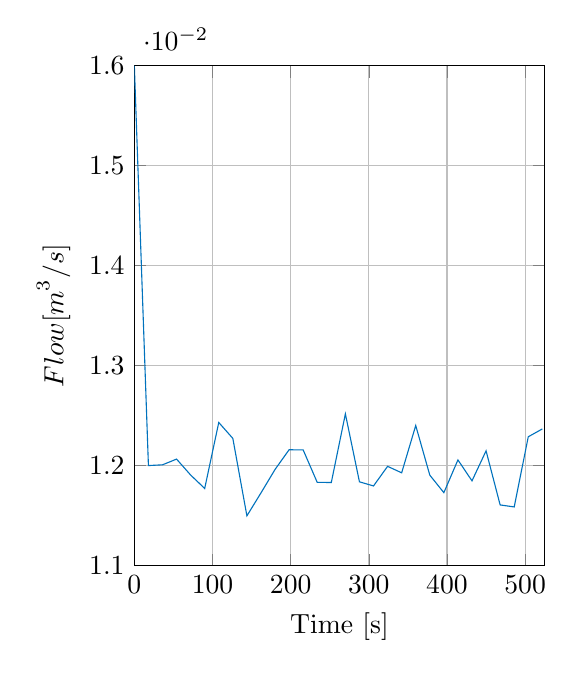
\begin{tikzpicture}

\begin{axis}[%
width=2.0517in,
height=2.5in,
at={(0.762in,0.481in)},
scale only axis,
%scaled ticks=base 10:2,
% scaled y ticks = false,
% y tick label style={/pgf/number format/fixed},
% /pgf/number format/1000 sep = \thinspace,
xmin=0,
xmax=525,
xlabel={Time [s]},
xmajorgrids,
ymin=0.011,
ymax=0.016,
ylabel={$\text{Flow [m}^\text{3}\text{/s]}$},
ymajorgrids,
axis background/.style={fill=white}
]
\addplot [color=mycolor1,solid,forget plot]
  table[row sep=crcr]{%
0	0.016\\
18	0.012001864965076\\
36	0.0120092762833444\\
54	0.0120664188872393\\
72	0.0119072901832867\\
90	0.0117729578654724\\
108	0.0124326877633298\\
126	0.0122734769119272\\
144	0.0114989740303722\\
162	0.0117284516956586\\
180	0.0119629523424902\\
198	0.0121600020489627\\
216	0.012157968696184\\
234	0.0118332199417125\\
252	0.0118328451738214\\
270	0.0125183003083703\\
288	0.0118392103354998\\
306	0.011797997025556\\
324	0.0119940759626088\\
342	0.0119292885666807\\
360	0.0124020000815428\\
378	0.0119060367921044\\
396	0.0117310579795223\\
414	0.012058217376743\\
432	0.0118489672188554\\
450	0.0121489715322212\\
468	0.0116081566208661\\
486	0.0115880976513915\\
504	0.0122897397953823\\
522	0.0123682266854666\\
};
\end{axis}
\end{tikzpicture}%
  \caption{}
  \label{fig:simulation_output_flow_height_a}
\end{subfigure}%
\begin{subfigure}{.4\textwidth}
  \centering
 % This file was created by matlab2tikz.
%
%The latest updates can be retrieved from
%  http://www.mathworks.com/matlabcentral/fileexchange/22022-matlab2tikz-matlab2tikz
%where you can also make suggestions and rate matlab2tikz.
%
\definecolor{mycolor1}{rgb}{0.00000,0.44700,0.74100}%
%
\begin{tikzpicture}

\begin{axis}[%
width=2.0521in,
height=2.566in,
at={(0.758in,0.481in)},
scale only axis,
xmin=0,
xmax=525,
xlabel={Time [s]},
xmajorgrids,
ymin=0.093,
ymax=0.098,
change y base=true,
y SI prefix=centi,
ylabel={Water height [cm]},
ymajorgrids,
axis background/.style={fill=white}
]
\addplot [color=mycolor1,solid,forget plot]
  table[row sep=crcr]{%
0	0.0951502385266159\\
18	0.095111043227792\\
36	0.0948226977069577\\
54	0.0945153779876514\\
72	0.0940524851393103\\
90	0.094875993427114\\
108	0.0972211389655122\\
126	0.0954652401379945\\
144	0.093158557787308\\
162	0.0932957050227688\\
180	0.0943627774415008\\
198	0.0951697376677062\\
216	0.0949084612329712\\
234	0.0936279623087843\\
252	0.0953273368751663\\
270	0.0978338003674198\\
288	0.0953215576000356\\
306	0.0942897420214976\\
324	0.0949588978631447\\
342	0.0953402059352639\\
360	0.0960242063423523\\
378	0.0946957433400719\\
396	0.0947824594720997\\
414	0.0946780388723197\\
432	0.0937119376701837\\
450	0.0948966891692525\\
468	0.0942014195796334\\
486	0.093465905053025\\
504	0.0958083762806446\\
522	0.0960549059718411\\
};
\end{axis}
\end{tikzpicture}%
  \caption{}
   \label{fig:simulation_output_flow_height_b}
\end{subfigure}
\caption{(a) Output flow, (b) the water height at the output of the channel.}
\label{fig:simulation_output_flow_height}
\end{figure}
\fxnote{Paa den her test skal der skrives hvad der testes paa, diameter, hoejde, healdning osv.}
These figures shows that whether the height is increasing or decreasing the flow is following, which is what is expected, because a higher water level will result in a higher flow rate and vice versa.
